\documentclass[11pt]{article}
\usepackage{graphicx}


\begin{document}

\title{Assignment 1}
\maketitle

\begin{flushright}

Group Details:
\break
\break
Santosh Kumar Desai
\\
2017H1030130P
\break
\break
Hritik Soni
\\
2014A2PS0480P
\break
\break
\end{flushright}


\section{Parallel Sieve of Eratosthenes}
The source can be located inside a folder called source in Q1 directory.\\
A Readme file has also been provided.\\

\noindent How to run:\\

\noindent mpicc primeFinder.c -lm\\
mpirun -np 2 a.out\\



\noindent For Cluster Execution (Utilities are provided inside utilities folder)\\

\noindent 1. Set up passwordless ssh\\
2. Populate all the hosts in the hosts\_file and host\_file\_slots.\\
3. Use provided Makefile to generate the executable.\\
4. Run copy\_program.sh to copy the executable to every host.\\
5. Execute mpirun -np 8 -hostfile host\_file\_slots a.out \\

\noindent Results\\

\noindent For an interactive plot, open Erato.html inside Graphs folder\\

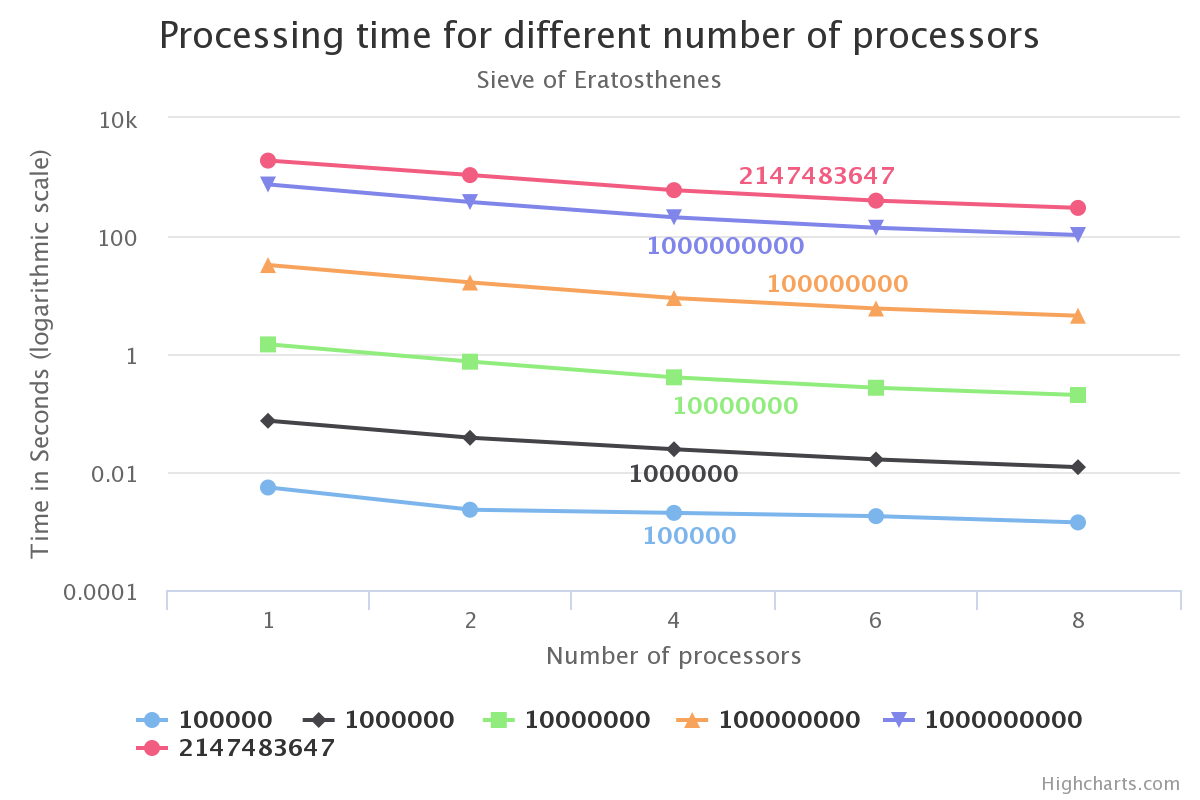
\includegraphics[width=\textwidth]{Graphs/Sieve.png}

\section{Distributed Indexer}

\noindent The source can be located inside a folder called source in Q2 directory.\\

\noindent The Program is divided into three seperate programs.\\

\noindent 1. docMaker.cpp - Arbitrary sized random documents generator implemented as a MPI program.\\

\noindent The generated executable needs to run on every node and it will automagically create all the documents as per specified in the source.\\
To create documents it randomly picks words from a specified wordlist until the specified wordcount is reached.\\

\noindent To change the number of documents created and the size of each document, modify docwlen and docn variables inside docMaker.cpp appropriately.\\

\noindent The convention for naming documents is "doc-i" where i goes from 0 to n-1 where n is document count.\\

\noindent 2. indexer.cpp - Local index generator for every node.\\

\noindent The indexer reads each document word by word and stores the count, document name along with the freuqency of each word in the form of a hashtable.\\
Finally, the hash table is written persistently in a file named index.\\

\noindent The format of each index is - Lots of Lines where each line contains information about a single word\\
word freq0 nodeid0 docid0 freq1 nodeid1 docid1 ... and so on\\
The frequencies are stored in descending order.\\

\noindent So, in summary using this index we can instantly locate where exactly most occurence of it exists, second most occurence and so on.   \\

\noindent 3. indexMerger.cpp - Global index generator by merging all local indices implemented as an MPI Program.\\

\noindent It works by merging indices step by step until all are merged and final index is stored at Process 0.\\

\noindent An illustration is shown below:\\

\noindent Consider 4 machines\\

\noindent 0 1 2 3\\

\noindent In first step index0 and index1 are merged and at the same time index2 and index3 are also merged.\\
This is done by 1 sending its index to 0 and 3 sending to 2.\\
So we are left with the following nodes:\\

\noindent 0   2\\

\noindent Now in the second step 2 sends it index to 0 and 0 merges its own index with 2's index.\\

\noindent 0\\

\noindent Finally, we are left with 0 and this index stores the global index.\\

\noindent The format is the same as that of local index.\\


\noindent For Cluster Execution (Utilities are provided inside utilities folder)\\

\noindent 1. Set up passwordless ssh\\
2. Populate all the hosts in the hosts\_file.\\
3. Use provided Makefile to generate the three executables - docMaker, indexer and indexMerger.\\
4. Run copy\_program.sh to copy the executables, wordlist and stopwordlist to every host.\\
5. Execute the three executables manually using mpirun or use the provided run.sh file.\\

\noindent Results\\

\noindent For an interactive plot, open Map-Reduce.html inside Graphs folder.\\

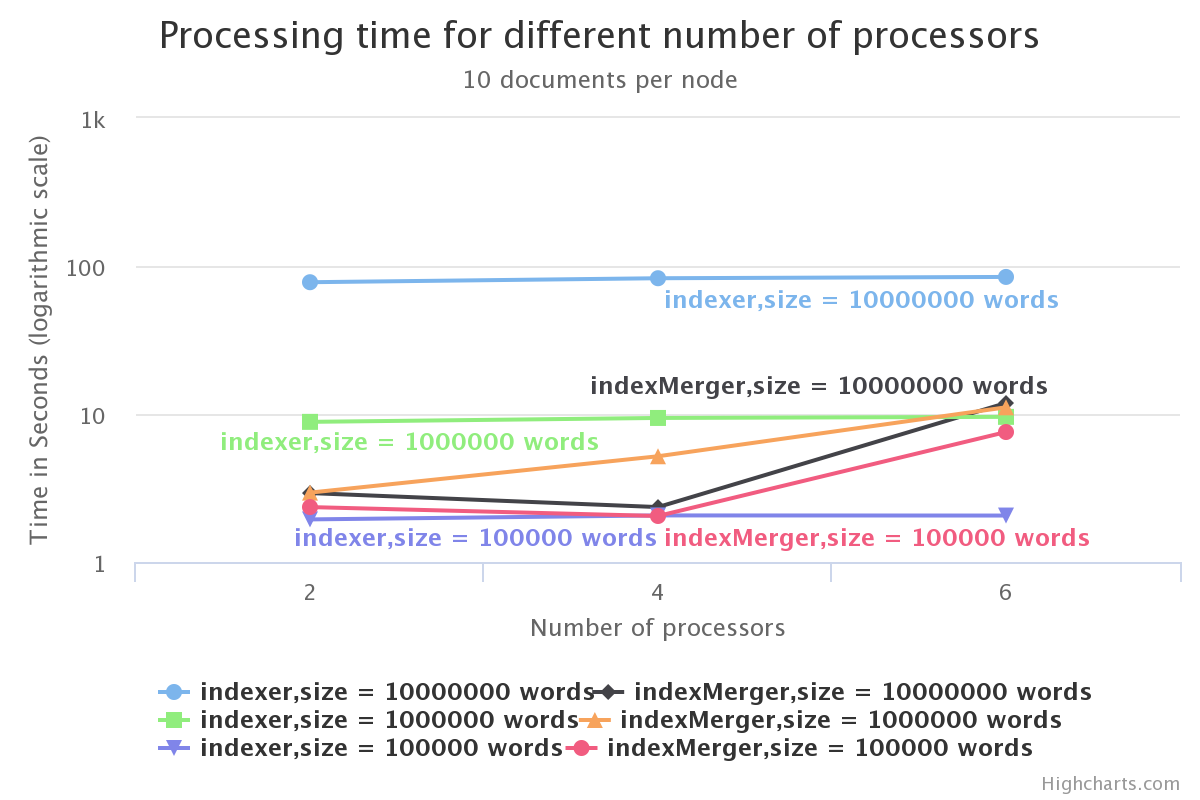
\includegraphics[width=\textwidth]{Graphs/Map-Reduce.png}


\end{document}
